\documentclass[dvipdfmx,11pt]{beamer}

\usepackage{bxdpx-beamer}% dvipdfmxなので必要
\usepackage{listings,jlisting}%ソースコード貼り付けのため
\usepackage{tikz}
\usepackage{otf}
\usetikzlibrary{positioning}
\usetikzlibrary{shadows}
\AtBeginDvi{\special{pdf:tounicode 90ms-RKSJ-UCS2}} %% しおりが文字化けしないように
\setbeamertemplate{navigation symbols}{} %% 右下のアイコンを消す

\renewcommand{\kanjifamilydefault}{\gtdefault}

\usetheme{Warsaw}
%\usetheme{Darmstadt}

\setbeamertemplate{footline}[frame number] %% スライド下のバーを消してフレーム番号を表示
\useoutertheme{shadow}                 %% 箱に影をつける
\usefonttheme{professionalfonts}       %% 数式の文字を通常の LaTeX と同じにする

\usepackage{graphicx,xcolor}%%文字の色
%\usepackage{bm}

\lstset{
	%プログラム言語(複数の言語に対応,C,C++も可)
 	language = Python,
 	%背景色と透過度
 	backgroundcolor={\color[gray]{.90}},
 	%枠外に行った時の自動改行
 	breaklines = true,
 	%自動開業後のインデント量(デフォルトでは20[pt])	
 	breakindent = 10pt,
 	%標準の書体
 	basicstyle = \ttfamily\scriptsize,
 	%basicstyle = {\small}
 	%コメントの書体
        commentstyle = \ttfamily\scriptsize,
 	%commentstyle = {\itshape \color[cmyk]{0,0,0,1}},
 	%関数名等の色の設定
 	classoffset = 0,
 	%キーワード(int, ifなど)の書体
 	keywordstyle = {\bfseries \color[cmyk]{0,1,0,0}},
 	%""で囲まれたなどの"文字"の書体
 	stringstyle = {\ttfamily \color[rgb]{0,0,1}},
 	%枠 "t"は上に線を記載, "T"は上に二重線を記載
	%他オプション:leftline,topline,bottomline,lines,single,shadowbox
 	frame = TBrl,
 	%frameまでの間隔(行番号とプログラムの間)
 	framesep = 5pt,
 	%行番号の位置
 	numbers = left,
	%行番号の間隔
 	stepnumber = 1,
	%右マージン
 	%xrightmargin=0zw,
 	%左マージン
	%xleftmargin=3zw,
	%行番号の書体
 	numberstyle = \tiny,
	%タブの大きさ
 	tabsize = 4,
 	%キャプションの場所("tb"ならば上下両方に記載)
 	captionpos = t
}

\title{解集合プログラミングを用いた\\ハミルトン閉路問題の解法に関する考察}
\author{平手 貴大(101730309)}
\institute{名古屋大学情報学部コンピュータ科学科情報システム系\\番原研究室}
\date{2020年度 卒業研究発表会\\2021年2月19日}

\begin{document}
%%%%%%%%%%%%%%%%%%%%%%%%%%%%%%%%%%%%%%%%%%%%%%%%%%%%%%%%%%%%%%%%%%%

\frame{\maketitle}
%%%%%%%%%%%%%%%%%%%%%%%%%%%%%%%%%%%%%%%%%%%%%%%%%%%%%%%%%%%%%%%%%%%

\begin{frame}{ハミルトン閉路問題(Hamiltonian Cycle Problem)}
  \begin{itemize}
  \item \alert{ハミルトン閉路問題}
    \begin{itemize}
    \item 与えられたグラフの全頂点をちょうど一度ずつ
      通る閉路が存在するかどうかを判定する問題.
    \item 始点と終点が一致するという閉路の条件を
      取り除けば,ハミルトン路問題となる.
    \end{itemize}
  \item \alert{最短ハミルトン閉路問題}
    \begin{itemize}
    \item グラフの辺に距離が付随しているときに
      最短距離のハミルトン閉路を求める問題.
    \end{itemize}
  \item \alert{コスト制約付きハミルトン閉路問題}
    \begin{itemize}
    \item ハミルトン閉路問題に,距離の総和が所与の閾値以下
      (または以上)であることを制約条件として付加した問題.
    \end{itemize}
  \end{itemize}
  \begin{alertblock}{}
    本研究では,無向グラフ上のハミルトン閉路問題
    およびその関連問題を対象とする.    
  \end{alertblock}
\end{frame}
%%%%%%%%%%%%%%%%%%%%%%%%%%%%%%%%%%%%%%%%%%%%%%%%%%%%%%%%%%%%%%%%%%%

\begin{frame}{コスト制約付きハミルトン閉路問題}
  \begin{figure}[tb]
  \centering
  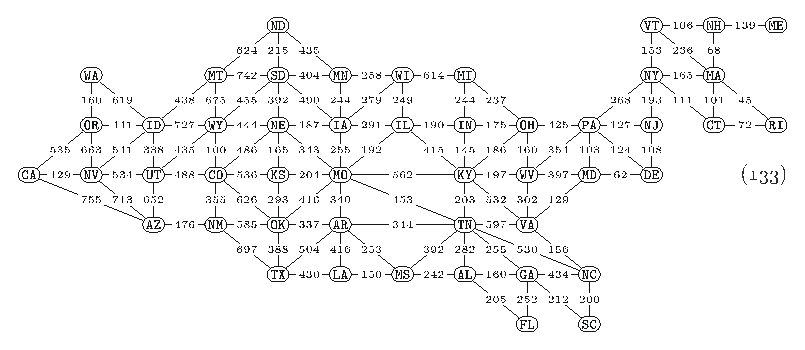
\includegraphics[width=0.8\linewidth]{fig/taocp_vol4fasc1b_p52_eq133.pdf}
  \caption{D.~E.~Knuth の教科書にある最短ハミルトン路問題の例}
  \end{figure}

  \begin{itemize}
  \item WA から ME までのハミルトン路は 6,876,928 通り
    あり,最短ハミルトン路は 11698 マイル.
  \item WA から ME までの距離の総和がある閾値以下である
    ハミルトン路を求める問題.
  \item 閾値を最短距離の 10\%増 (12,868 マイル) とした場合,
    解の総数は 16180 個.
  \end{itemize}
   
\end{frame}
%%%%%%%%%%%%%%%%%%%%%%%%%%%%%%%%%%%%%%%%%%%%%%%%%%%%%%%%%%%%%%%%%%%

\begin{frame}{解集合プログラミング(Answer Set Programming)}
  \begin{itemize}
  \item \alert{ASP 言語}は,一階論理に基づく知識表現言語の一種.
  \item \alert{ASP システム}は論理プログラムから
    安定モデル意味論に基づく解集合を計算するシステム.
  \item 近年,SAT 技術を応用した高速 ASP システムが開発され,
    スケジューリング,プランニング,システム生物学,システム検証,
    制約充足問題,制約最適化問題など様々な分野への実用的応用が急速に拡大している.
  \end{itemize}

  \begin{alertblock}{ハミルトン閉路問題に ASP を用いる利点}
    \begin{itemize}
    \item ASP 言語は表現力が高く,制約の記述が容易.
    \item 組み込みの非閉路制約を利用できる.
    \item 高速な解列挙.
    \end{itemize}
  \end{alertblock}
\end{frame}
%% %%%%%%%%%%%%%%%%%%%%%%%%%%%%%%%%%%%%%%%%%%%%%%%%%%%%%%%%%%%%%%%%%%%

\begin{frame}{研究目的}
  \begin{alertblock}{研究目的}
  ASP 技術を活用し,大規模なハミルトン閉路問題を
    効率よく解く手法を模索する.
  \end{alertblock}
  \begin{block}{研究内容}
    \begin{itemize}
    \item \structure{ハミルトン閉路問題を解く3種類の ASP 符号化を考案.}
      \begin{itemize}
      \item 3つの符号化 \textsf{undirected}, \textsf{directed}, \textsf{acyclicity}.
      \item 最短ハミルトン閉路問題,コスト制約付きハミルトン閉路問題へ拡張.
      \end{itemize}
    \item \structure{既存のベンチマーク問題集を用いた評価実験.}
      \begin{itemize}
      \item  ベンチマーク問題は7種類,計517問.
      \item ハミルトン閉路問題に対する実験.
      \item 最短ハミルトン閉路問題に対する実験.
      \item コスト制約付きハミルトン路問題に対する実験.
      \end{itemize}
    \end{itemize}
  \end{block}
\end{frame}
%%%%%%%%%%%%%%%%%%%%%%%%%%%%%%%%%%%%%%%%%%%%%%%%%%%%%%%%%%%%%%%%%%%

\begin{frame}{提案する ASP 符号化}
  \begin{block}{ハミルトン閉路問題の表現}
    与えられた無向グラフ$G= (V,E)$上に,以下の2つの制約を満たす
    部分グラフ$G'= (V,E')$が存在するか判定する問題.
    \begin{itemize}
    \item $G'$の各頂点の次数が2.(次数制約)
    \item $G'$が連結である.(連結制約)
    \end{itemize}
  \end{block}
  \begin{itemize}
  \item \alert{\textsf{undirected}符号化}
    \begin{itemize}
    \item ハミルトン閉路問題を次数制約と連結制約で簡潔に表現した符号化.
    \end{itemize}
  \item \alert{\textsf{directed}符号化}
    \begin{itemize}
    \item \textsf{undirected}符号化をベースに,与えられた無向グラフを
      有向グラフ化して解く符号化.
    \end{itemize}
  \item \alert{\textsf{acyclicity}符号化}
    \begin{itemize}
    \item \textsf{directed}符号化をベースに,連結制約に代わり
      部分閉路を禁止する制約を使用.
      \item ASPの$\#edge$宣言で部分閉路を禁止する制約を簡潔に表現.
    \end{itemize}
  \end{itemize}
\end{frame}
%%%%%%%%%%%%%%%%%%%%%%%%%%%%%%%%%%%%%%%%%%%%%%%%%%%%%%%%%%%%%%%%%%%

\begin{frame}{実験概要}
  %%  提案した符号化の性能を評価するために実験を行った.
  以下では,提案した符号化の性能を評価するために行った実験について2つ説明する.
  \begin{itemize}
  \item \structure{比較する ASP 符号化}:
    \begin{itemize}
    \item \textsf{undirected}符号化
    \item \textsf{directed}符号化
    \item \textsf{acyclicity}符号化
    \end{itemize}
  \item \structure{対象とする問題}:
    \begin{itemize}
    \item ハミルトン閉路問題
      \begin{itemize}
      \item \structure{制限時間}: 30分
      \item \structure{オプション}: \textit{trendy}
      \item \structure{ベンチマーク問題}:\\
        \textsf{color04},
        \textsf{complete},
        \textsf{knight},
        \textsf{tsplib},
        \textsf{grid},
        \textsf{random}
      \end{itemize}
    \item コスト制約付きハミルトン閉路問題(解の全列挙)
      \begin{itemize}
      \item \structure{制限時間}: 3時間
      \item \structure{オプション}: \textit{crafty}
      \item \structure{ベンチマーク問題}: \textsf{usmap} (閾値: 10問)
      \end{itemize}
    \end{itemize}
  \item \structure{ASP システム}: \textit{clingo-5.4.0}
  \item \structure{実験環境}: Mac mini Intel Corei7 3.2GHz, 64GBメモリ
  \end{itemize}
\end{frame}
%%%%%%%%%%%%%%%%%%%%%%%%%%%%%%%%%%%%%%%%%%%%%%%%%%%%%%%%%%%%%%%%%%%

\begin{frame}{ハミルトン閉路問題の実験結果(解けた問題数)}
%%%%%%%%%%%%%%%%%%%%%%%%%%%%%%%%%%%%%%%%%%%%%%%
\begin{table*}[t]\footnotesize
  \centering
% \tabcolsep = 0.8mm
% \renewcommand{\arraystretch}{1.2}
  \begin{tabular}{lr||r|r|r}
    頂点数 & 問題数 & \textsf{undirected} & \textsf{directed} & \textsf{acyclicity}\\
   \hline
    $\:\:\:\:\:\,\, 0 \leq |V| < 1000$  & 171   & 156   & \textbf{171}   & 155  \\
    $1000 \leq |V| < 2000$  & 165   & 120   & \textbf{158}   & 124  \\
    $2000 \leq |V| < 3000$  & 177   & 125   & \textbf{162}   & 73   \\
    $3000 \leq |V| < 4000$  & 185   & 104   & \textbf{148}   & 42   \\
    $4000 \leq |V| < 5000$  & 128   & 92    & \textbf{104}   & 28   \\
    $5000 \leq |V| < 6000$  & 80    & 63    & \textbf{68}    & 23   \\
    $6000 \leq |V| < 7000$  & 55    & 39    & \textbf{43}    & 21   \\
    $7000 \leq |V| < 8000$  & 28    & 12    & \textbf{14}    & 5    \\
    $8000 \leq |V| < 9000$  & 10    & 2     & \textbf{5}     & 1    \\
    $9000 \leq |V| < 10000$ & 2     & \textbf{2}     & \textbf{2}     & 1    \\
   \hline
    合計 & 1001 & 715   & \textbf{875}   & 473  
  \end{tabular}
  \vskip .5em
  \caption{ハミルトン閉路問題: 解けた問題数}
  \label{sat_table}
\end{table*}
%label{sat_table}
%%%%%%%%%%%%%%%%%%%%%%%%%%%%%%%%%%%%%%%%%%%%%%%

\begin{itemize}
\item \textsf{S+U}では,\textsf{undirected} と \textsf{acyclicity} が,
  \textsf{directed} よりも2問多く解いた.
\item \textsf{SAT}では,\textsf{undirected} が,最も多くの問題を解いた.
\item \textsf{UNSAT}では,\textsf{directed} と \textsf{acyclicity} 符号化が,
  \textsf{undirected} より1問多く解いた.
\end{itemize}
\end{frame}
%%%%%%%%%%%%%%%%%%%%%%%%%%%%%%%%%%%%%%%%%%%%%%%%%%%%%%%%%%%%%%%%%%%

\begin{frame}{ハミルトン閉路問題の実験結果(カクタスプロット)}
%%%%%%%%%%%%%%%%%%%%%%%%%%%%%%%%%%%%%%%%%%%%%%%
\begin{figure}[tb]
\begin{center}
  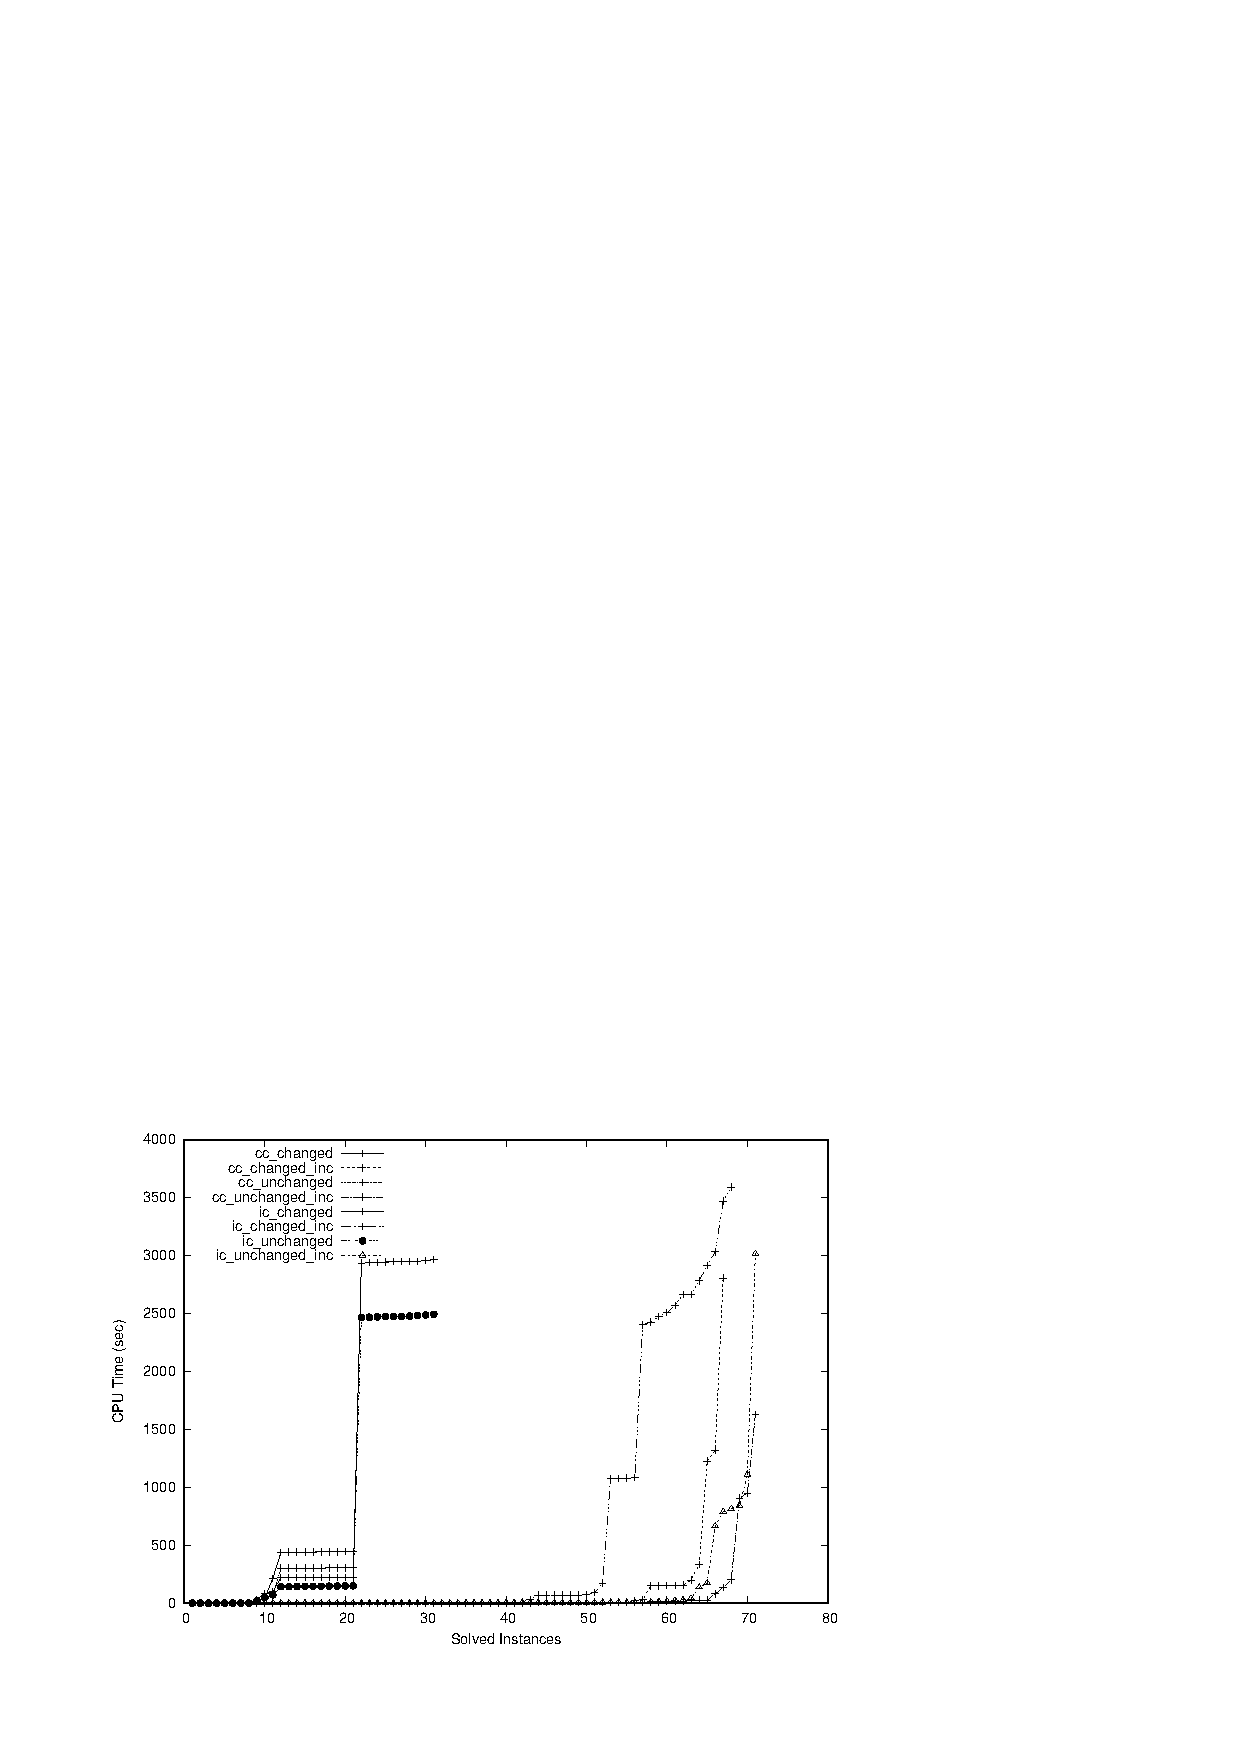
\includegraphics[width=0.7\linewidth]{fig/cactus.png}
%\caption{ハミルトン閉路問題: カクタスプロット (\textsf{SAT+UNSAT})}
\label{cactus}
\end{center}
\end{figure}
%%%%%%%%%%%%%%%%%%%%%%%%%%%%%%%%%%%%%%%%%%%%%%%

\begin{itemize}
\item \textsf{acyclicity}符号化は,
  解けた問題数が同じ\textsf{undirected}符号化と比較して,
  より高速に問題を解いていることが確認できた.
\end{itemize}
\end{frame}
%%%%%%%%%%%%%%%%%%%%%%%%%%%%%%%%%%%%%%%%%%%%%%%%%%%%%%%%%%%%%%%%%%%

\begin{frame}{コスト制約付きハミルトン閉路問題の実験結果}
%%%%%%%%%%%%%%%%%%%%%%%%%%%%%%%%%%%%%%%%%%%%%%%
\begin{table}[htbp]
  \caption{実験結果3}
  \label{cost_table}
  \centering
  \begin{tabular}{|l|r|rrr|}
    \hline
    制約Cost値    &	Models & undirected & directed & acyclicity \\
    \hline
    11698   &	1      &\textcolor{red}{2.919} &10.020 & 4.355	\\
    11814   &	8      &5.458  &7.416	& \textcolor{red}{4.136}	\\
    11931   &	28     &\textcolor{red}{3.226}&10.317	& 4.799	\\
    12282   &	388    &\textcolor{red}{9.993}&15.787	& 10.715	\\
    12867   &	16180  &16.386       &23.406	& \textcolor{red}{10.819}\\
    14037   &	939209 &47.894       &41.515	& \textcolor{red}{24.655}\\
    15207   &	4525541&85.256       &56.953	& \textcolor{red}{41.217}\\
    16377   &	6702964&93.595       &51.991	& \textcolor{red}{41.301}	\\
    17547   &	6876526&91.750       &46.065	& \textcolor{red}{37.290}	\\
    18716   &	6876928&95.659       &45.416	& \textcolor{red}{37.905}	\\
    \hline
    Average &   & 45.2136 & 30.889  & \textcolor{red}{21.7192}\\
    Best    &   & 3 & 0 & \textcolor{red}{7} \\
    \hline
  \end{tabular}
\end{table}
%\label{cost_table}
%%%%%%%%%%%%%%%%%%%%%%%%%%%%%%%%%%%%%%%%%%%%%%%

\begin{itemize}
\item \textsf{acyclicity}符号化が,より多くの問題を
  高速に解き,平均CPU時間も最も短かった.
\end{itemize}
    
\end{frame}
%%%%%%%%%%%%%%%%%%%%%%%%%%%%%%%%%%%%%%%%%%%%%%%%%%%%%%%%%%%%%%%%%%%

\begin{frame}{まとめ}
  \begin{block}{まとめ}
    \begin{itemize}
    \item \structure{ハミルトン閉路問題を解く3種類の ASP 符号化を考案.}
      \begin{itemize}
      \item ASP の高い表現力による,最短ハミルトン閉路問題,コスト制約付きハミルトン閉路問題への自然な拡張.
      \end{itemize}
    \item \structure{既存のベンチマーク問題集を用いた評価実験.}
      \begin{itemize}
      \item ハミルトン閉路問題とコスト制約付きハミルトン閉路問題について,
        \textsf{acyclicity}符号化の優位性が確認できた.
      \item 最短ハミルトン閉路問題については,
        \textsf{undirected}符号化の優位性を確認した.(本発表では省略)
      \end{itemize}
    \end{itemize}
  \end{block}
  \begin{alertblock}{今後の課題}
    \begin{itemize}
    \item SATソルバーを用いた既存研究で提案された,
      ハミルトン閉路問題をインクリメンタルに解く手法のASPを用いた実装.
    \item 巡回セールスマン問題への拡張.
    \end{itemize}
  \end{alertblock}
\end{frame}
%%%%%%%%%%%%%%%%%%%%%%%%%%%%%%%%%%%%%%%%%%%%%%%%%%%%%%%%%%%%%%%%%%%

\begin{frame}[noframenumbering]{}
  補足
\end{frame}
%%%%%%%%%%%%%%%%%%%%%%%%%%%%%%%%%%%%%%%%%%%%%%%%%%%%%%%%%%%%%%%%%%%

\begin{frame}{提案する符号化}
  \begin{itemize}
  \item 最短ハミルトン閉路問題への拡張
    \begin{itemize}
    \item 目的関数を追加.
    \item ハミルトン閉路上の辺に付与された距離の総和を最小化.
    \end{itemize}
  \item コスト制約付きハミルトン閉路問題への拡張
    \begin{itemize}
    \item コスト制約を追加.
    \item ハミルトン閉路上の辺の距離の総和が閾値以下である.
    \end{itemize}
  \end{itemize}
\end{frame}
%%%%%%%%%%%%%%%%%%%%%%%%%%%%%%%%%%%%%%%%%%%%%%%%%%%%%%%%%%%%%%%%%%%


\end{document}
